% ---------------------------------------------------------------------------
% Author guideline and sample document for EG publication using LaTeX2e input
% D.Fellner, v1.13, Nov 13, 2007

\documentclass{egpubl}

% --- for  Annual CONFERENCE
\VisualComputing % VisualComputing (added by U. Schwanecke, 2021)
%\ThreeDAnimation % 3DAnimation (added by U. Schwanecke, 2020)
%\Seminar % Specialist Seminar (added by U. Schwanecke, 2019)
%\ConferenceSubmission % uncomment for Conference submission
%\ConferencePaper      % uncomment for (final) Conference Paper
%\STAR                 % uncomment for STAR contribution
% \Tutorial             % uncomment for Tutorial contribution
% \ShortPresentation    % uncomment for (final) Short Conference Presentation
%
% --- for  CGF Journal
% \JournalSubmission    % uncomment for submission to Computer Graphics Forum
% \JournalPaper         % uncomment for final version of Journal Paper
%
% --- for  CGF Journal: special issue
% \SpecialIssueSubmission    % uncomment for submission to Computer Graphics Forum, special issue
% \SpecialIssuePaper         % uncomment for final version of Journal Paper, special issue
%
% --- for  EG Workshop Proceedings
% \WsSubmission    % uncomment for submission to EG Workshop
% \WsPaper         % uncomment for final version of EG Workshop contribution
%
%\electronicVersion % can be used both for the printed and electronic version

% !! *please* don't change anything above
% !! unless you REALLY know what you are doing
% ------------------------------------------------------------------------

\PrintedOrElectronic

\usepackage[pdftex]{graphicx} 
\usepackage{t1enc, dfadobe}
%\usepackage[T1]{fontenc}
\usepackage{egweblnk}
\usepackage{cite}

% For backwards compatibility to old LaTeX type font selection.
% Uncomment if your document adheres to LaTeX2e recommendations.
% \let\rm=\rmfamily    \let\sf=\sffamily    \let\tt=\ttfamily
% \let\it=\itshape     \let\sl=\slshape     \let\sc=\scshape
% \let\bf=\bfseries

% end of prologue

\usepackage{blindtext}
\usepackage{caption}
\usepackage{subfigure}
\usepackage{dblfloatfix}
\usepackage{adjustbox}
\usepackage{mathtools}
\usepackage{todonotes}


% ---------------------------------------------------------------------
\captionsetup{labelfont=bf,textfont=it}
\title[Fancy 3D Animation Demo]%
      {Fancy Paper in the Field of Visual Computing}

\author[U. Schwanecke]
    {\parbox{\textwidth}
        {\centering 
			U. Schwanecke
        }
        \\
    {\parbox{\textwidth}
        {\centering RheinMain University of Applied Sciences, Wiesbaden, Germany\\
       }
    }
}
% ------------------------------------------------------------------------

% if the Editors-in-Chief have given you the data, you may uncomment
% the following five lines and insert it here
%
% \volume{36}   % the volume in which the issue will be published;
% \issue{1}     % the issue number of the publication
% \pStartPage{1}      % set starting page


%-------------------------------------------------------------------------
\begin{document}

%-------------------------------------------------------------------------
% uncomment for using teaser (comment if you don't want a teaser)
\teaser{
    \hspace{\fill}
    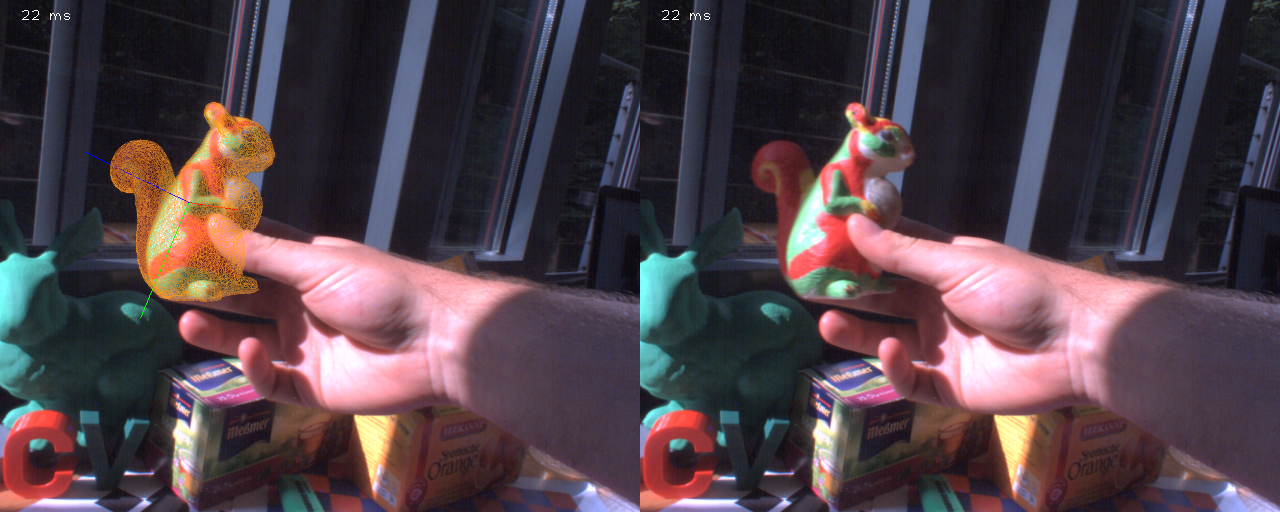
\includegraphics[width=0.9\linewidth]{images/ModelbasedTrackingExample.png}
    \hspace{\fill}
    \centering
    \caption{Best teaser image you can provide \ldots}
    \label{fig:teaser}
}


%-------------------------------------------------------------------------
\maketitle


%-------------------------------------------------------------------------
\begin{abstract}
Some informative abstract \ldots
\blindtext
\end{abstract}  


%-------------------------------------------------------------------------
\section{Introduction}
\label{sec:introduction}
Some nice introduction, e.g. citing some literature such as \cite{Tjaden2017, Achenbach2018, Sommer2020} \ldots 

$$
\sum_{i=1}^n i = \frac{n(n+1)}{2}
$$
\blindtext


%-------------------------------------------------------------------------
\section{Related Work}
\label{sec:related_work}
Maybe a separate section about related work \ldots 
\blindtext


%-------------------------------------------------------------------------
\section{Approach}
\label{sec:approach}
\blindtext


%-------------------------------------------------------------------------
\section{Experiments}
\label{sec:Experiments}
\blindtext


%-------------------------------------------------------------------------
\section{Conclusions}
\label{sec:conclusion}
Some famous last words \ldots
\blindtext


%-------------------------------------------------------------------------
\section{Acknowledgements}
\label{sec:acknowledgements}
Maybe you like to acknowledge \ldots 


%-------------------------------------------------------------------------
%\bibliographystyle{eg-alpha}
\bibliographystyle{eg-alpha-doi}
\bibliography{paper-bib}

\end{document}